\section{节点表示学习}
在第\ref{Intro}节中,我们谈到,浅层的node embedding是一类较为简单的图表示学习方法,而其中比较具有代表性的就是\emph{DEEPWALK}、\emph{LINE}以及\emph{node2vec},因此,在本节中,我们将简要介绍这三种node embedding方法。

\subsection{\emph{DEEPWALK}}
\emph{DEEPWALK}是由Perozzi等\cite{perozzi2014deepwalk}提出的一个非常经典的节点表示学习方法,其核心思想是将network embedding与自然语言处理中极为重要的word embedding方法word2vec联系起来,从而将network embedding问题转换成了一个word embedding问题。

\begin{figure}[!htbp]
  \centering
  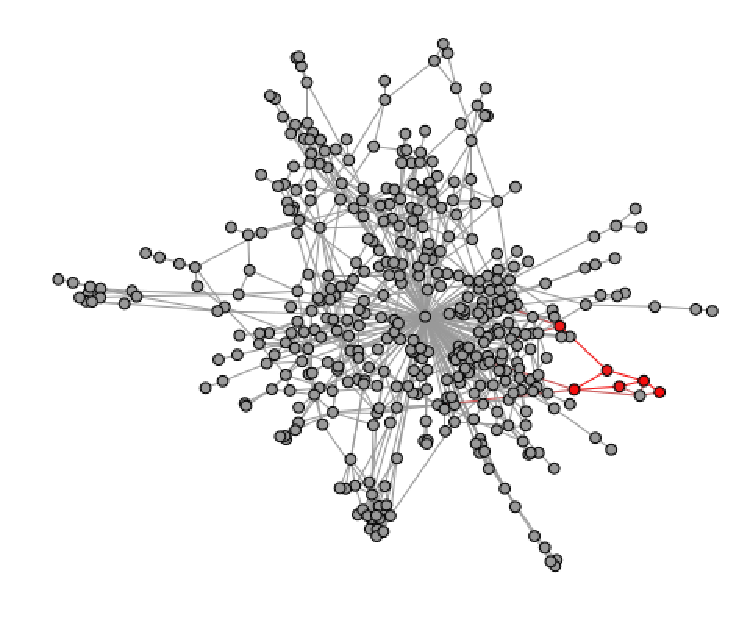
\includegraphics[scale=1]{Fig/randomwalk.pdf}
  \caption{随机游走生成示意图\cite{perozzi2014deepwalk}}
  \label{fig:randomwalk}
\end{figure}

\emph{DEEPWALK}算法由两个主要的部分组成。前一部分是随机游走生成器。\emph{DEEPWALK}从每一个节点出发$\gamma$次,每一次都采取均匀采样的方式选择当前节点的邻接节点作为下一步的节点随机游走,当游走的路径长度达到$t$之后,停止一次游走。按照这种方式便可以生成一个个节点游走序列,每个序列称为一个\emph{walk},如图\ref{fig:randomwalk}所示。每个\emph{walk}被当作word2vec中的一个句子,而每个节点即为word2vec中的一个词。而算法的第二部分即为将语言模型SkipGram应用到随机游走生成的\emph{walk}上面,使用大小为$w$的滑动窗口作为一个walk的context,使用一个context的中心节点去推测context中的所有其它节点。因此,目标函数即为
\[\min_{\Phi}-\log{Pr}(\{v_{i-w}, \cdots, v_{i-1}, v_{i+1}, \cdots, v_{i+w}\}\mid \Phi(v_i))\]
其中,$\Phi$为映射函数$\Phi: v\in V\mapsto \mathbb{R}^{|V|\times d}$

在实验环节,\emph{DEEPWALK}选择多标签分类作为评价算法性能的指标。评价中将通过\emph{DEEPWALK}学习获得的embedding按照不同的比例划分为训练集和测试集,训练集作为$N$个\emph{one-vs-rest}对率回归分类器的训练数据,将其中置信度最高的$k$个类别作为节点的预测类别。其中,$N$为类别的个数,$k$为节点的表签数。

\subsection{\emph{LINE}}
\emph{DEEPWALK}通过随机游走的方式,将图结构数据转化为了自然语言处理的任务来完成。然而,在图结构数据中,节点之间的关系比词上下文的关系更为复杂;而且,图结构数据中的边通常具有权重,使用现有的word2vec方法无法很好的应对这个问题;另外,在真实数据中,图的规模通常过于庞大,存下所有的\emph{walk}将会带来巨大的开销。

Tang等\cite{tang2015line}提出了一种新的network embedding方法:\emph{LINE}。该算法适用于各种类型的图,如有向图、无向图、有权图和无权图,并且能够支持百万节点的图。而且,该算法能够同时保留节点的一阶相似度和二阶相似度。

\begin{figure}[!htbp]
  \centering
  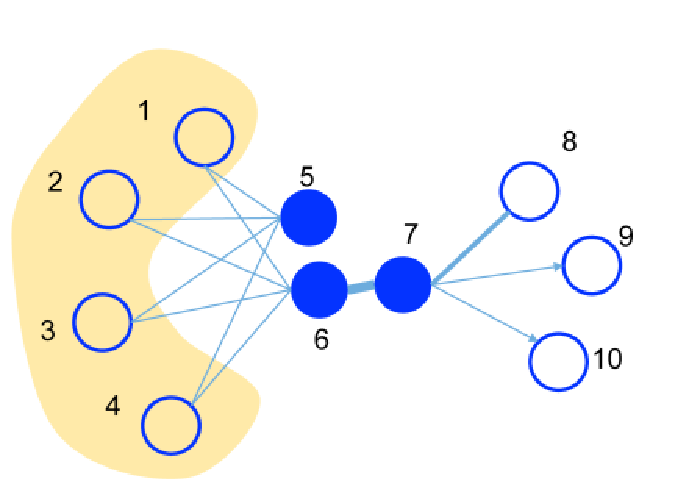
\includegraphics[scale=1]{Fig/line.pdf}
  \caption{一阶相似度和二阶相似度示意图\cite{tang2015line}}
  \label{fig:line}
\end{figure}

一阶相似度是两个顶点之间的局部成对相似度。对于由边$(u, v)$相连的一对节点来说,边的权重$w_{uv}$即为$u$和$v$的一阶相似度,如果两个节点之间没有边相连,那么一阶相似度即为0。换句话说,一阶相似度就是两个节点直接联系的紧密程度,保留一阶相似度就是保留节点之间的边权。例如,图\ref{fig:line}中的节点$6$和$7$之间有一条权重很大的边相连,因此这两个节点之间具有非常大的一阶相似度,所以当映射到低维空间之后,这两个节点应该离得很近。

二阶相似度是一对节点的邻居网络结构之间的相似度。从数学上来说,令$p_u=(w_{u, 1}, \cdots, w_{u,|V|})$表示节点$u$和其它所有节点的一阶相似度,则节点$u$和$v$的二阶相似度即为$p_u$和$p_v$的相似度。如果没有任何节点同时与$u$和$v$相连,那么它们之间的二阶相似度即为0。例如,图\ref{fig:line}中的节点$5$和$6$尽管没有边相连,但是它们有许多公共邻居,也就是具有很高的二阶相似度,因此这两个节点的低维表示也应该离得很近。

在\emph{LINE}中,两个节点实际的一阶相似度定义如下
\[\hat{p}_1(i, j) = \frac{w_{ij}}{W}\]
其中,$W$是所有边权重之和。而两个节点embedding的相似度定义为
\[p_1(v_i, v_j) = \frac{1}{1+ \exp(-\stackrel{\rightarrow}{u}_i^T\cdot \stackrel{\rightarrow}{u_j})}\]
其中,$\stackrel{\rightarrow}{u_i}\in R^d$是节点$v_i$在低维向量空间的embedding。目标函数设为实际相似度与表示相似度之间的$KL$散度,这样一来,只要最小化KL散度(下式中约去了一些常数),就能保证表示相似度尽量接近实际相似度:
\[O_1 = -\sum_{(i, j)\in E}w_{ij}\log p_1(v_i, v_j)\]
需要注意的是,一阶相似度仅适用于无向图,通过最小化上述目标函数,就可以找到每一个节点在$d$维空间的表示。

二阶相似度既适用于无向图,也适用于有向图。两个节点实际的二阶相似度定义如下
\[\hat{p}_2(v_j|v_i) = \frac{w_{ij}}{d_i}\]
其中,$w_{ij}$是边$(v_i, v_j)$的权重,$d_i$是节点$v_i$的出度。两个节点的embedding相似度定义为
\[p_2(v_j|v_i) = \frac{\exp(\stackrel{\rightarrow}{u'}_j^T\cdot \stackrel{\rightarrow}{u_i})}{\sum_{k=1}^{|V|}\exp(\stackrel{\rightarrow}{u'}_k^T\cdot \stackrel{\rightarrow}{u_i})}\]
其中,$V$为节点$v_i$的所有邻居。与一阶相似度不同的是,对于邻居节点,使用了另一组embedding,称为context。目标函数依旧为$KL$散度:
\[O_2 = -\sum_{(i, j)\in E}w_{ij}\log p_2(v_j\mid v_i)\]

最终要获得同时包含有一阶相似度和二阶相似度的embedding,只需要将通过一阶相似度获得的embedding与通过二阶相似度获得的embedding拼接即可。

实验证明,当考虑了一阶相似度之后,\emph{LINE}在节点分类任务中的效果要好于\emph{DEEPWALK}。

\subsection{\emph{node2vec}}
Node2Vec\cite{grover2016node2vec}是一份基于DeepWalk的延伸工作,它改进了DeepWalk随机游走的策略。在网络中的节点和边缘上的预测任务需要在学习算法所使用的工程特征方面花费精力。最近在更广泛的表征学习领域的研究通过学习特征本身在自动化预测方面取得了重大进展。在Node2vec中,学习了节点到特征的低维空间的映射,这最大化了保留节点的网络邻域的可能性。定义了节点网络邻域的灵活概念,并设计了一个有偏差的随机游走过程,有效地探索了不同的邻域。这也是该算法的主要贡献。该算法推广了基于网络邻域的严格概念的先前工作,并且作者认为探索邻域的额外灵活性是学习更丰富表示的关键。

DeepWalk中根据边的权重进行随机游走,而Node2Vec加了一个权重调整参数$\alpha$,最终生成的随机序列是一种DFS和BFS的结合,模型仍使用$skip gram$去训练,其中DFS和BFS是经典的查找策略。Node2Vec方法认为,现有的方法无法很好的保留网络的结构信息,例如图\ref{fig:node2vec1}所示,有一些点之间的连接非常紧密(比如$u, s1, s2, s3,s4$),他们之间就组成了一个社区(community)。网络中可能存在着各种各样的社区,而有的结点在各个社区中可能又扮演着相似的角色(比如$u$与$s6$)。

\textbf{基本假设}:\textbf{为了}使得优化问题易于处理,给出了两个标准假设:
1.条件独立,2.特征空间的对称性。

优化目标:让同一个社区内的结点表示能够相互接近,或在不同社区内扮演相似角色的结点表示也要相互接近。

\begin{figure}[!htbp]
	\centering
	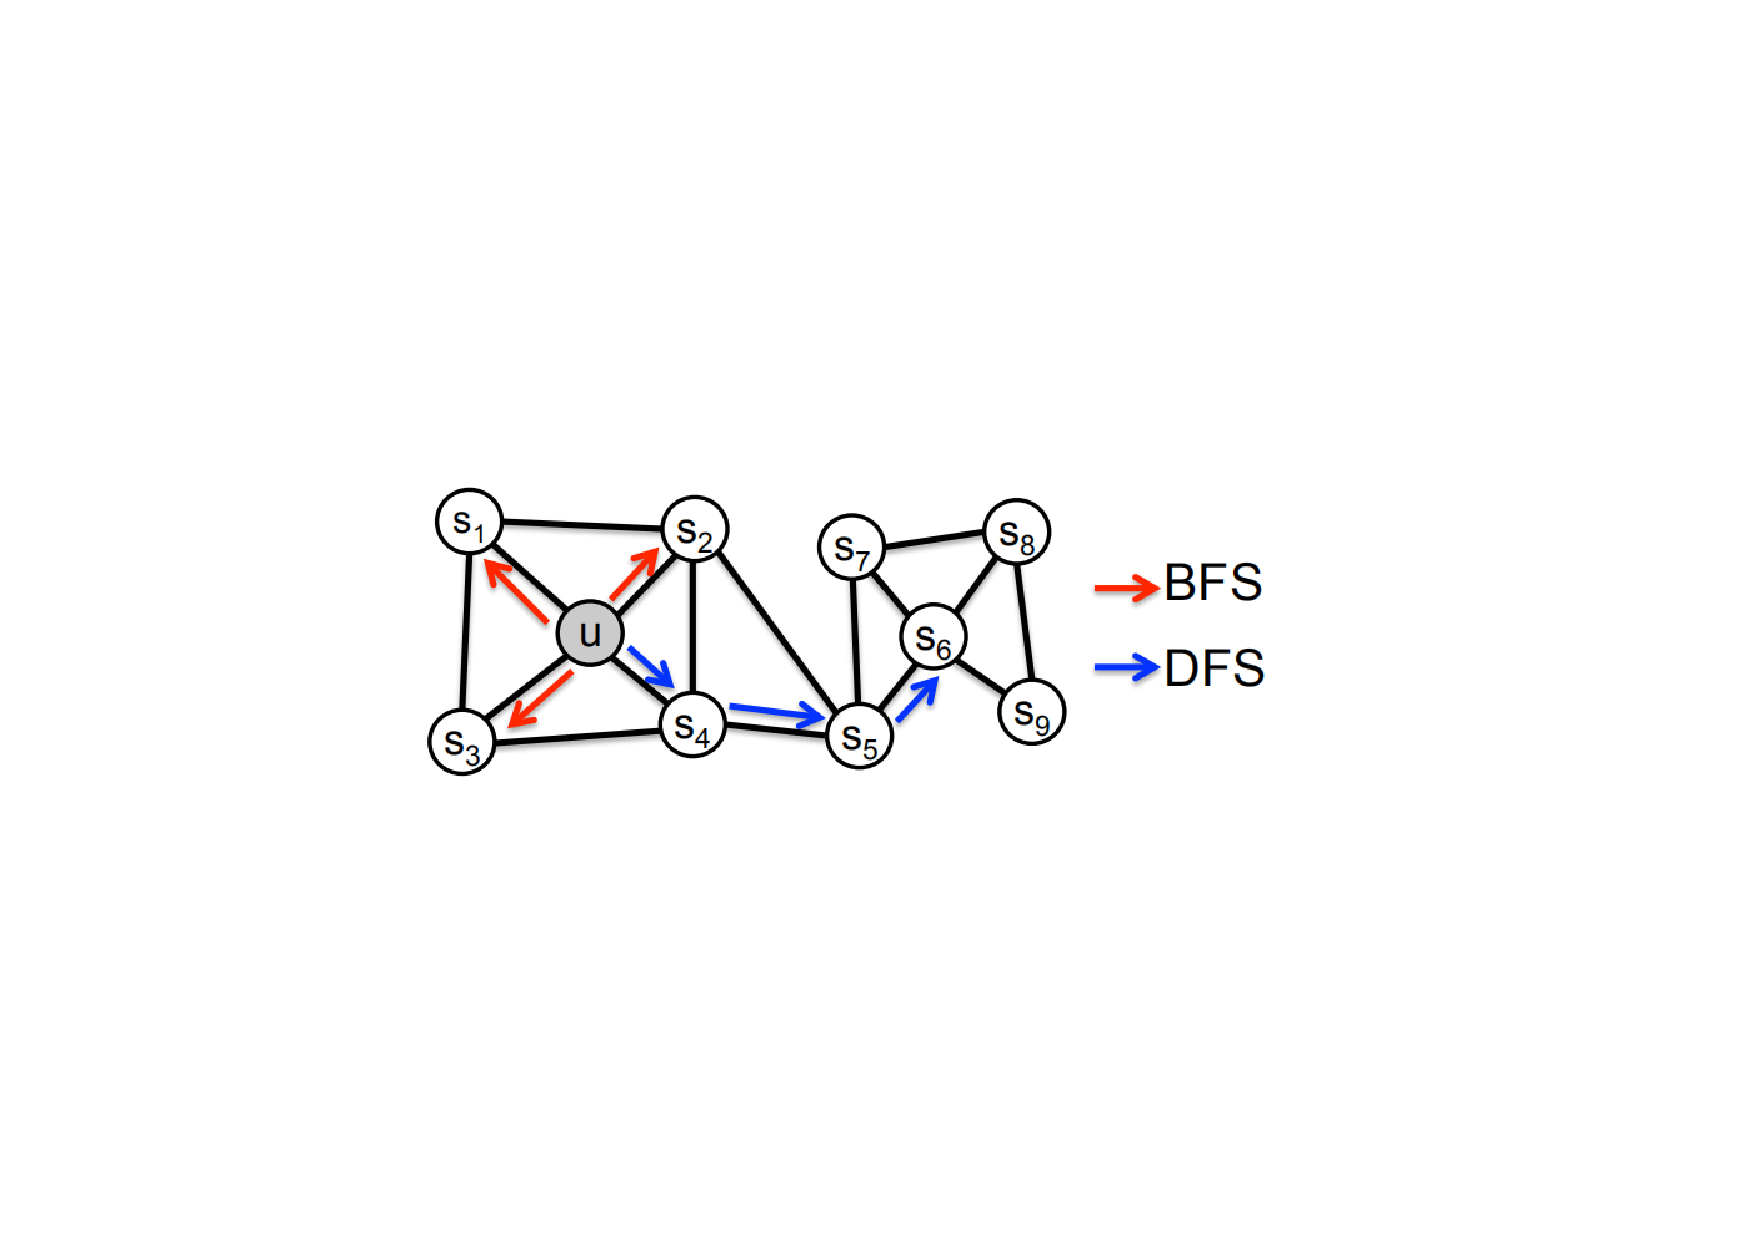
\includegraphics[scale=1]{Fig/Node2Vec_1.pdf}
	\caption{BFS和DFS从节点$u$开始的搜索策略\cite{grover2016node2vec}}
	\label{fig:node2vec1}
\end{figure}

\textbf{方法简述}:

1.随机游走

给定一个起始节点$u$,我们模拟一个固定长度l的随机游走,$c_i$表示行走中的第$i$个节点,起始节点:$c_0 = u$。节点$c_{i-1}$走到节点$c_i$概率定义为:

$$ P(c_i=x|c_{i-1}=v)=\left\{
\begin{aligned}
\dfrac{\pi_{uv}}{Z} & if (u,v)\in E\\
0 & otherwise
\end{aligned}
\right.
$$

$\pi_{vx}$是节点之间非归一化概率;Z是节点之间概率的和,作为归一化因子。

2.寻找偏差$\alpha$

假设已知游走路径已从$t$走到$v$,从节点$v$ 走到下一个节点$x$按照转移概率$\pi_{vx}$选择对应的节点;$\pi_{vx}=\alpha_{ p q}(t,x)·w_{vx}$,如图\ref{fig:node2vec2}所示

\begin{figure}[!htbp]
	\centering
	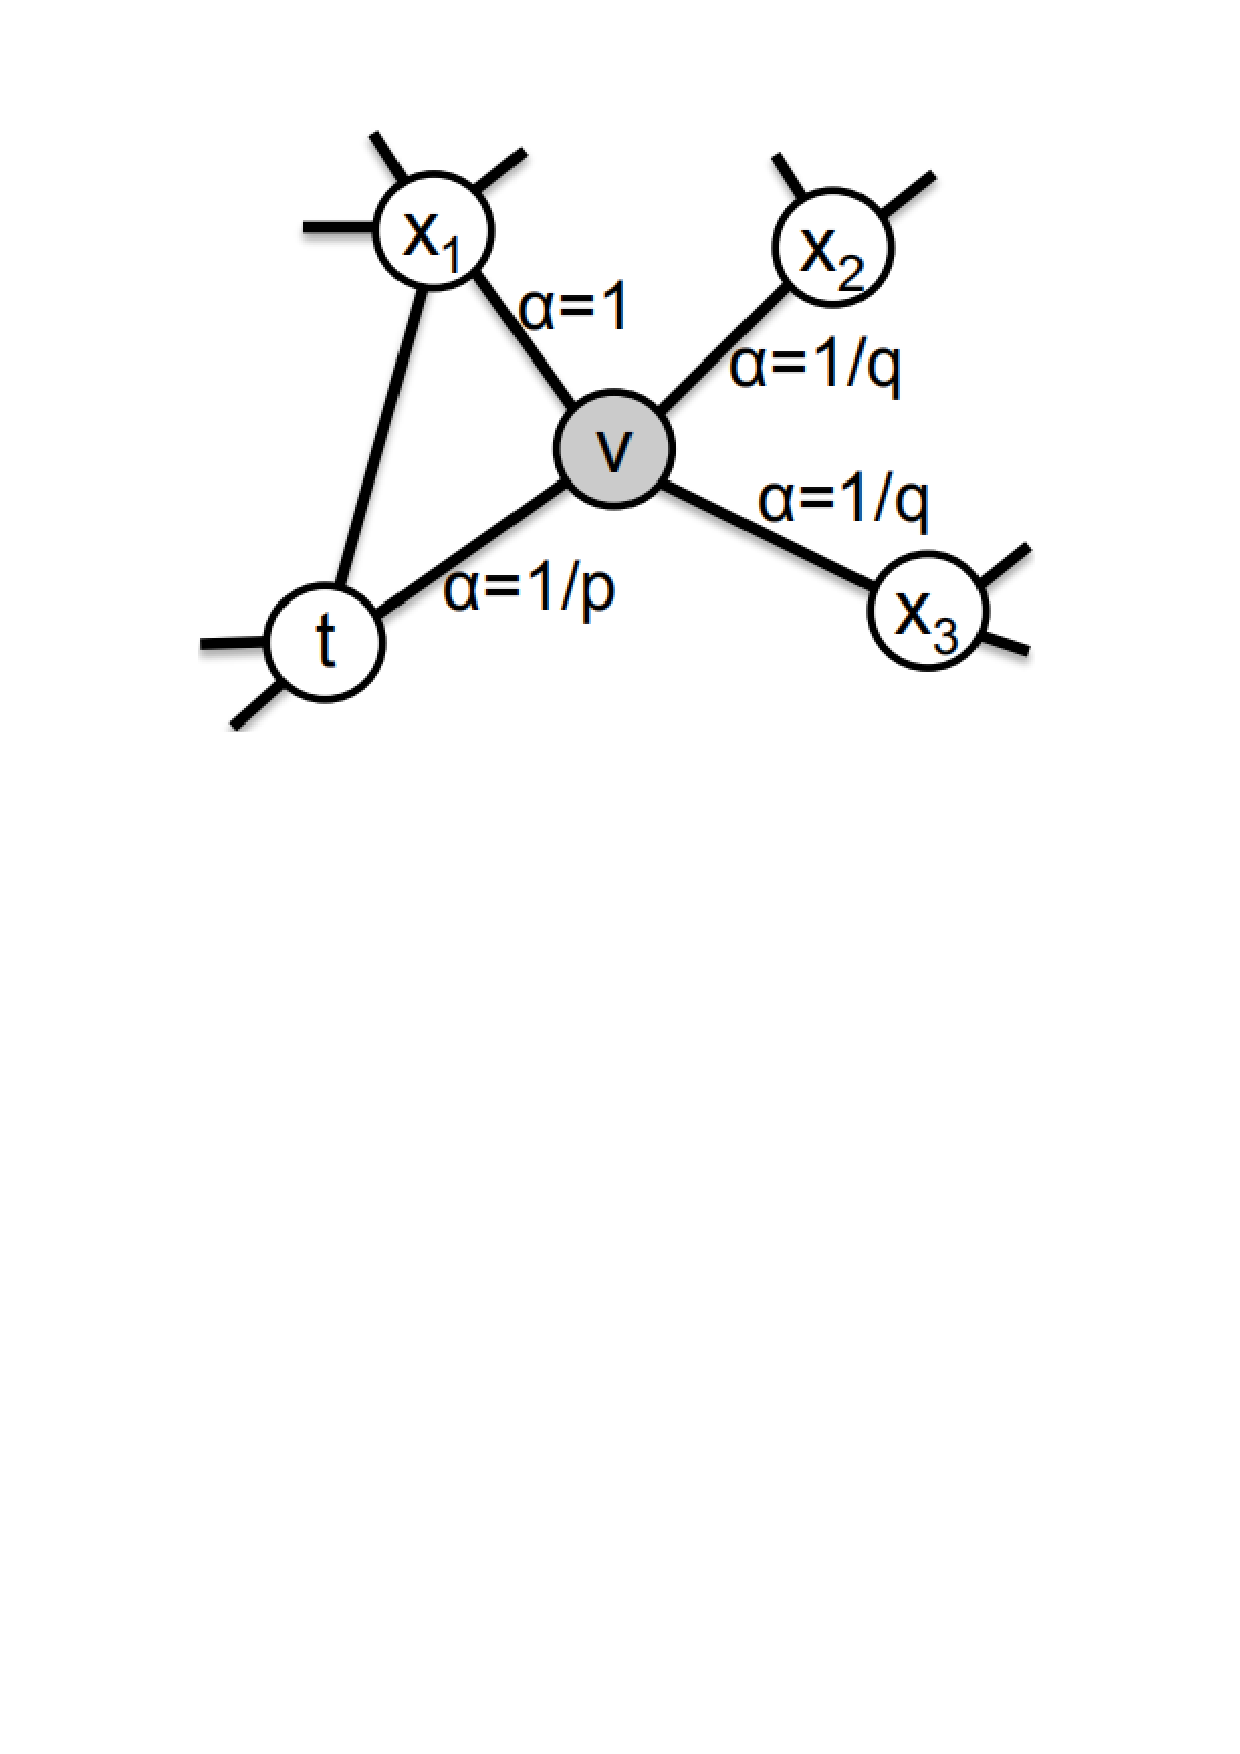
\includegraphics[scale=1]{Fig/Node2Vec_2.pdf}
	\caption{在node2vec中随机游走的说明\cite{grover2016node2vec}}
	\label{fig:node2vec2}
\end{figure}

其中,$d_{tx}$是$t$到$x$的最近距离。在论文中,$d_{tx}$的取值为[0 1 2]。$p,q$这两个参数决定离开起始节点的速度。

参数$p$:

1.表示访问已遍历节点的可能性;

2.$p > max(q, 1)$:表示在连续两步,越小的可能访问已遍历节点;这种策略鼓励适度的探索,并避免了距离为2的节点抽样中的冗余

3.$p < min(q, 1)$:表示遍历的节点接近起始节点;

参数$q$

1.允许搜索区分“向内”和“向外”节点;

2.$q>1$:表示越大的可能抽样节点靠近$t$;可以获得与遍历中的开始节点相关的底层图的局部视图,与BFS类似;

3.$q<1$:表示越大的可能抽样节点远离$t$,与DFS类似;

4.$p=q=1$就是deepwalk


Node2vec伪代码

\begin{tabular}{l}
	\hline
	
	\textbf{Algorithm 1} The node2vec algorithm.\\
	
	\textbf{LearnFeatures} (Graph $G = (V, E, W)$, Dimensions $d$, Walks \\per node $r$, Walk length $l$, Context size $k$, Return $p$, In-out $q$)\\
	
	$\pi$ = PreprocessModifiedWeights($G, p, q$)\\
	
	$G0 = (V, E, π)$\\
	
	Initialize walks to Empty\\
	
	\textbf{for} iter = 1 \textbf{to} $r$ \textbf{do}\\
	
	\quad \textbf{for all} nodes $u \in V $\textbf{do}\\
	
	\quad\quad $walk$ = node2vecWalk($G0, u, l$)\\
	
	\quad\quad Append $walk$ $to$ $walks$\\
	
	$f$ = StochasticGradientDescent($k, d, walks$)\\
	
	return $f$\\
	\hline 
	
	\textbf{node2vecWalk} (Graph $G0 = (V, E, \pi])$, Start node $u$, Length $l$)\\
	
	Inititalize $walk$ to $[u]$	\\
	
	\textbf{for} $walk\_iter$ = 1 to $l$ \textbf{do}	\\
	
	\quad$curr$ = walk[1]	\\
	
	\quad$Vcurr$ = GetNeighbors($curr, G0$) $s$ = AliasSample($Vcurr, \pi$)\\
	
	\quad Append $s$ to $walk$	\\
	
	\textbf{return} $walk$	\\
	\hline   
	
\end{tabular}


